\section{Extended methods and audit contract}
\subsection{Attempt linkage and source limits}
\label{app:provenance}
The inventory contains one score-selected record per decoder episode, not one observation per archived attempt. Earlier or superseded attempts are retained in the private archive and are not counted again. The 704 historical rows lack attempt identifiers; readers select the last matching untagged record. All 704 archived decoder-source strings match their corresponding score rows. Report objects match in all 541 cases where one was archived; 163 lack such an object. These checks cannot distinguish historical reruns that produced identical outputs.

Two damaged gzip archives yielded 27 complete selected records before compression errors. Their stored decoder and report fields were checked against the score rows, but the recovered data are not checksum verified. For the 56 fresh episodes, score and event hashes are verified. Failed fresh decoder subtypes use a later work-folder source snapshot that was not bound into the original attempt hashes. Accordingly, stored pass scores are authoritative, while these subtype attributions are provisional.

Newer harness paths bind an attempt identifier into the score and transcript, flush the archive before atomically replacing the score table, and refuse stale derived labels. This protects single-writer crash recovery; it does not provide transactional coordination between concurrent writers. The present paper does not retrospectively assign attempt identifiers to historical records.

\subsection{Ground truth and diagnostic attributes}
The simulator plants fault scope, stationarity, mechanism, and changed physical qubits. For a reported qubit set $Q_r$ and true changed set $Q_t$, localization is
\begin{equation}
J(Q_r,Q_t)=\frac{|Q_r\cap Q_t|}{|Q_r\cup Q_t|}.
\end{equation}
The localization gate requires $J\geq0.5$ on local or moving faults. Reporting every qubit is therefore penalized when the fault is genuinely local. The report's adequacy classification and mechanism accuracy are retained separately. The headline diagnosis criterion checks scope, stationarity, and applicable localization; it does not add mechanism correctness after observing the results. A local report marked nonstationary is accepted for a moving fault under the stored equivalence.

The oracle uses the true simulator noise and shotwise regimes. It is privileged relative to the agent and does not establish optimal decoding. The custom nonstationary reference searches a hypothesis bank constructed for the benchmark grammar using the pre-drift circuit, a simulation seed, and detector data. It is neither information-matched to an arbitrary general agent nor an independently reproduced adaptive decoder from the literature. Reference gates establish decoding headroom; they do not prove that every diagnosis field is statistically identifiable from a finite deployment batch.

\subsection{Frozen visible-only baseline}
\label{app:baseline}
Adequacy compares deployment detector means with 20,000 nominal simulated shots (seed 0). The statistic is the maximum absolute mean difference divided by $\sqrt{p(1-p)(1/n+1/m)}$, where $p$ is the pooled detector rate clipped to $[10^{-4},0.9999]$. The complete statistic is calibrated with 99 whole-shot label permutations using seed 1. The p-value is $(1+\#\{T_{\rm null}\geq T_{\rm obs}\})/100$; inadequacy is reported at $p\leq0.01$.

Stationarity uses non-overlapping blocks of 32, 128, and 512 shots, retaining a scale only when at least four blocks fit. Each scale discards its incomplete final block and estimates detector means from its complete prefix. The statistic is the maximum standardized block deviation over eligible scales, blocks, and detectors. Ninety-nine whole-shot order permutations (seed 2) calibrate the complete statistic, with inclusive ties and the same truncation. Fewer than 128 shots are unsupported. This measures order dependence, not every possible nonstationary latent process.

For an inadequate model, localization unions qubits in adaptive-bank hypotheses assigned to at least 50 deployment shots. The complete bank is retained, including hypotheses not selected during deployment. Indices outside the circuit's declared physical qubits are rejected. A union covering at least half of the circuit qubits is called global; otherwise it is local, including an empty union that can fail. An adequate model reports scope none. Confidence is fixed at 50; permutation p-values are not posterior confidence.

The baseline chooses nominal correlated matching for adequate models, pairwise-refit correlated matching for global faults, and the adaptive decoder for local faults. Its mechanism report is a fixed heuristic: none for adequate, all for local, and readout for global. Fitting runs in the no-network sandbox with a 3,600-second limit. Hidden decoder scoring has a fixed 300-second limit. Timeouts, unsupported cases, and exceptions remain in the all-candidate denominator. The 92 fresh candidates change locations and shot seeds inside selected families; they are not unseen-family tasks.

\section{Extended descriptive results}
\label{app:extended}
\begin{table*}[t]
\centering\small
\caption{Coverage of all 760 trajectory reviews. Rule columns retain the measured scoring/eligibility contract; review columns retain raw transcript annotations. The 47 earlier eligibility exclusions are preserved despite annotation disagreements. Earlier task contracts differ; this is an audit inventory, not a pooled model comparison.}
\begin{tabular}{lrrrrrr}\toprule
Population & Episodes & Rule included & Rule pass & Review pass & Review failure & Review excluded\\\midrule
Main evaluation &533&533&144&146&387&0\\
Earlier experiments &171&124&42&52&117&2\\
Fresh-seed evaluation &56&56&13&13&43&0\\
\midrule
All recorded episodes &760&713&199&211&547&2\\\bottomrule
\end{tabular}
\end{table*}

\begin{figure*}[t]
\centering
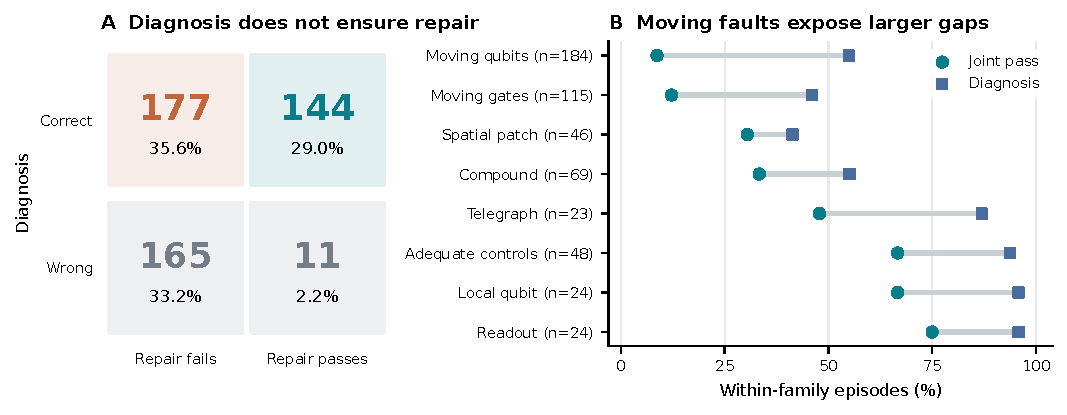
\includegraphics[width=\textwidth]{figures/diagnosis-repair.pdf}
\caption{\textbf{Diagnosis and repair are separate bottlenecks.} A: 497 scored development episodes; 36 unscored episodes remain headline failures. One unscored diagnosis is correct, giving 322/533 overall. B: family rates include unscored episodes. Shared tasks/configurations make rates descriptive. Independent Parquet/inventory checks match 533 rows and 144 passes, discrepancy zero.}
\label{fig:outcomes}
\end{figure*}

\subsection{Resource use and fresh-seed predictions}
The archived completed-tool-call counts cover all 533 development episodes. Among the 36 budget-exhausted episodes, 22 record 40 completed calls, four record 39, and ten record 41. The runner counts started calls for stopping and completed calls for the archived summary, so the nominal budget and final completed count are distinct. Some scored and successful episodes also approach the budget; the distribution alone cannot identify a harmful strategy or a benefit from additional calls.

Before fresh evaluation, predictions anticipated localization over-reporting, a possible dwell-time association, and expensive adaptive decoding. In the 80 localized baseline cases, 71 predicted more qubits than truth, six the same number, and three fewer. Mean predicted and true set sizes were 27.875 and 15.913; mean false-positive qubits were 12.063. The full baseline had 18 scoring timeouts. All 16 distance-7 candidates timed out, compared with two of 72 distance-5 and zero of four distance-9 candidates. Distance is confounded with template and decoder path, so this is not a scaling law.

For localized cases with an explicit trailing dwell, dwell 30 has 20 rows with mean/median localization 0.409/0.334; dwell 40 has eight with 0.649/0.632; and dwell 60 has 20 with 0.630/0.717. Longer-dwell groups exceed dwell 30, but mean and median are not monotonic across 40 and 60. The comparison remains confounded. It does not identify the causal effect of dwell.

The fresh baseline's hierarchical bootstrap uses 10,000 draws with frozen seed 20261108, resampling families, templates within families, and replicates within templates. Sampled clusters retain their original member count. Intervals are descriptive because there are few families and one episode per model/configuration/candidate does not estimate model-sampling variance. Fresh model execution is separately availability selected and sparse; its 13/56 relative passes must not be compared as a matched rate with the fully evaluated baseline.

\subsection{Rule--judge disagreement}
The seven current development disagreements are shown below. Four assignments imply sufficient repair despite a measured recovery below 0.5. We preserve the original judgments and measured outcomes rather than silently reconciling them.

\begin{table}[ht]
\centering\small
\caption{All development rule--judge disagreements. A dagger marks a measured repair-floor contradiction.}
\begin{tabular}{llr}\toprule
Rule leaf & Judge leaf & Count\\\midrule
Nominal unchanged & Plain fitted & 2\\
Plain fitted & Diagnosis failure$^\dagger$ & 1\\
Plain fitted & Passed$^\dagger$ & 1\\
Plain fitted & Under-adapted & 1\\
Under-adapted & Diagnosis failure$^\dagger$ & 1\\
Under-adapted & Passed$^\dagger$ & 1\\\bottomrule
\end{tabular}
\end{table}

Across all cohorts there are 60 disagreements. Forty-seven arise from an earlier environmental eligibility policy: a required-module import error excludes the episode even if the agent later recovers. All 47 traces contain that error, while the judge assigns 10 passes, 30 plain-fitted, three nominal-unchanged, two diagnosis-failure, one harmful, and one broken-decoder label. This is a retained historical eligibility dispute, not 47 newly established model capability failures. The remaining disagreements and current score contradictions prevent treating raw agreement as independent annotation accuracy.

\section{Literature boundary and reproducibility}
\label{app:artifacts}
The source-by-source novelty matrix covers adaptive QEC, learned decoding/control, quantum-code benchmarks, scientific agents, and trajectory/judge evaluation. The contribution remains the joint diagnosis-and-repair contract and audited corpus, not a new decoder or a universal first. The online SSI environment already tasks agents with surface-code decoder development: \url{https://openssi.dev/ssi-index/environments/surface-code-decoding/} (verified project artifact, not a paper). The main text cites the relevant primary papers; the source bundle records the detailed overlap and search queries.

All 20 bibliography entries were verified through primary records, actual paper PDFs, and DOI metadata. Journal publication records govern the journal citations; arXiv citations retain their preprint years. The bibliography does not invent a venue for a preprint. A source-by-source novelty matrix and search record accompany the source. Targeted retrieval through 11 November 2026 does not prove exhaustive novelty or a universal priority claim.

The public aggregate inputs reproduce the paper figures without private trajectories. The source bundle includes the exact plotting input, pinned plotting versions, reference verification records, upstream style provenance, and a hash manifest. Private identifiers, raw traces, and downloaded third-party paper PDFs are excluded. The official ICML 2026 style is used in preprint mode, with no submission or acceptance claim. The circulation version has four main-text pages; references and this appendix are outside that count. Individual workshops may require a different template, page track, or anonymized submission.
